\chapter{Aufgabe 1 }
\section*{a}
\subsection*{i}
Siehe Abbildung \ref{fig:graphLCOM}

\begin{figure}
	\centering
	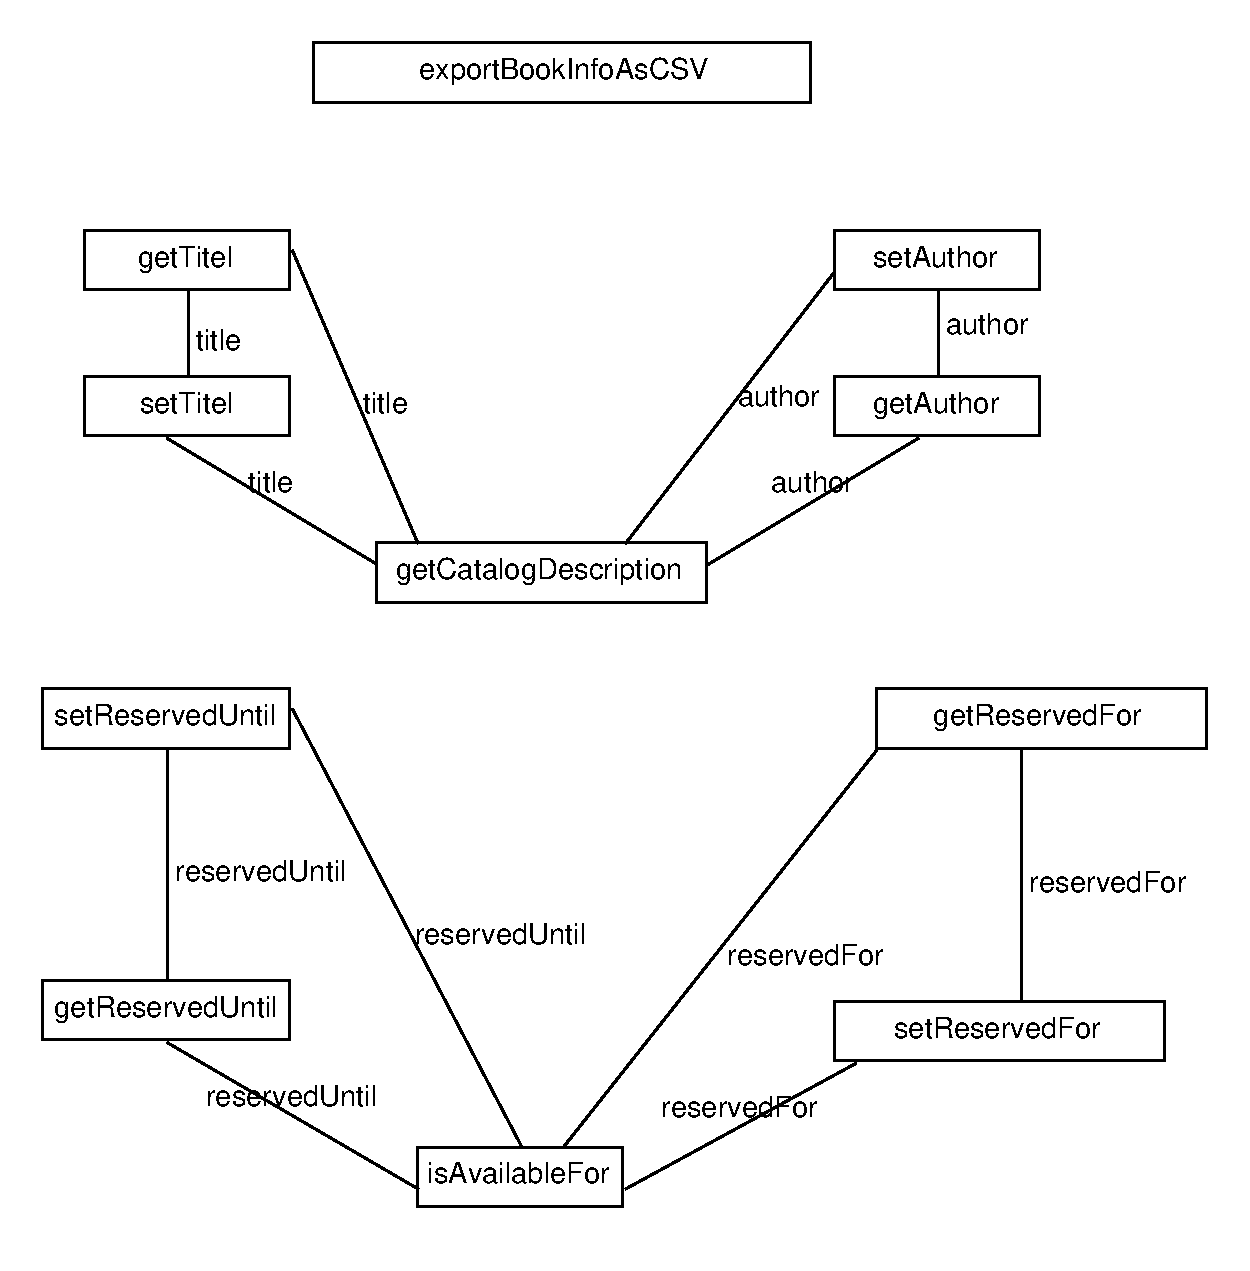
\includegraphics[width=0.8\textwidth, clip]{images/graphLCOM.pdf}
	\caption{Zusammenhangsgraph der Klasse Book für das  LCOM Verfahren. }
	\label{fig:graphLCOM}
\end{figure}
\subsection*{ii}
\textbf{LCOM = 3 von 11}



\section*{b}
Die Verantwortungen 


\section{c}
%	\lstset { %
%	language=java,
%	backgroundcolor=\color{black!5}, % set backgroundcolor
%	basicstyle=\footnotesize,% basic font setting
%}

\lstset{language=Java,
	showspaces=false,
	showtabs=false,
	breaklines=true,
	showstringspaces=false,
	breakatwhitespace=true,
}


\definecolor{dkgreen}{rgb}{0,0.6,0}
\definecolor{gray}{rgb}{0.5,0.5,0.5}
\definecolor{mauve}{rgb}{0.58,0,0.82}

\lstset{frame=tb,
	language=Java,
	aboveskip=3mm,
	belowskip=3mm,
	showstringspaces=false,
	columns=flexible,
	basicstyle={\small\ttfamily},
	numbers=none,
	numberstyle=\tiny\color{gray},
	keywordstyle=\color{blue},
	commentstyle=\color{dkgreen},
	stringstyle=\color{mauve},
	breaklines=true,
	breakatwhitespace=true,
	tabsize=3,
	backgroundcolor=\color{black!5},
	numbers=left, stepnumber=1, numberstyle = \tiny % set backgroundcolor
}
\begin{lstlisting}
	package org.library;
	
	import java.util.Date;
	
	import org.library.users.Client;
	
	public class Book implements LibraryItem {
		
		private String title;
		private String author;
		
		private Client reservedFor;
		private Date reservedUntil;    
		
		
		// getters an setters
		public String getTitle() {  return title; }
		public void setTitle(String title) { this.title = title; }
		
		public String getAuthor() { return author; }
		public void setAuthor(String author) { this.author = author; }
		
		public Client getReservedFor() { return reservedFor; }
		public void setReservedFor(Client reservedFor) { this.reservedFor = reservedFor; }
		
		public Date getReservedUntil() { return reservedUntil; }
		public void setReservedUntil(Date until) { this.reservedUntil = until; }
		
		// implementiert interface LibraryItem
		@Override
		public String getCatalogDescription() {
			return title + " by " + author;  
		}
		
		// prueft, ob Buch vom Kunden geliehen werden kann
		public boolean isAvailableFor(Client c, Date from) {
			if (reservedFor != null || reservedUntil.after(from)) {
				return false;
			}
			return c.numberOfBorrowedBooks() < 3;
		}
		
		// exportiert Buchinformation als csv Datei
		public void exportBookInfoAsCSV(org.library.formats.CSVExporter exporter) throws java.io.IOException {        
			exporter.writeLine(getTitle(), getAuthor());        
		}    
	}
\end{lstlisting}

